\section{项目架构}
此心理评测系统使用B/S架构,前端使用React框架搭建用户界面,后端使用Python的Flask Web框架搭建Restful API。

\subsection{项目目录}

好的项目目录有清晰的条理,可以通过目录知道各个文件夹的作用,易于拓展。

\subsubsection{前端项目目录}
\begin{figure}[thbp!]
	\centering
	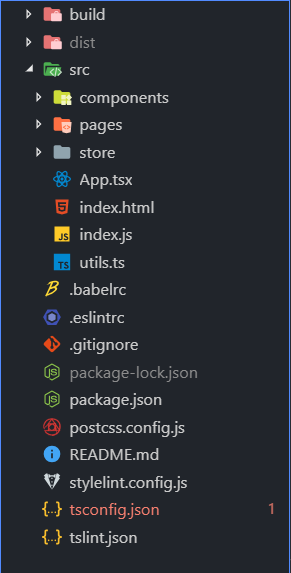
\includegraphics[width=0.3\linewidth]{figure/frontend_structure}
	\caption{前端项目目录}
	\label{fig:frontend_structure}
\end{figure}

build文件夹下存放着webpack的编译打包配置文件,分为两个环境,development开发环境和production生产环境。

dist文件夹是存放着webpack打包后的文件,用作于webpack-dev-server的开发环境文件和上线后的生产环境文件。

src文件夹是项目的根目录,里面的components文件夹存放着公用的组件,pages存放着系统的各个页面文件,store存放着项目所需要用到的redux状态仓库,App.tsx是项目的主页面,index.html是webpack打包注入js依赖的html文件,index.js是项目的主入口,utils.js是项目所需要的共用工具。

.babelrc是babel-loader的配置文件,配置编译js的目标版本。

.eslintrc是eslint代码检查的配置文件。

.gitignore是git仓库push的时候忽略的文件。

package.json是前端项目的架构文件,记载该前端项目所需要的依赖和依赖版本和该前端项目的基本信息。

postcss.config.js是postcss的配置文件。

README.md是描述该项目的markdown文件。

stylelint.config.js是stylelint css代码检查的配置文件。

tsconfig.json是Typescript的编译配置文件。

tslint.json是tslint的配置文件。

\subsubsection{后端项目目录}
\begin{figure}[thbp!]
	\centering
	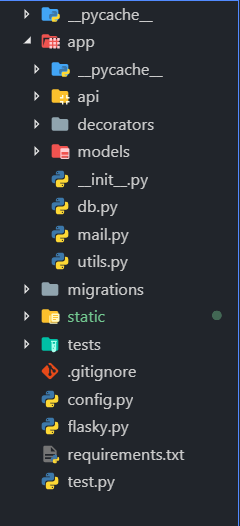
\includegraphics[width=0.3\linewidth]{figure/backend_structure}
	\caption{后端项目目录}
	\label{fig:backend_structure}
\end{figure}

\_\_pycache\_\_是IDE自动生成的sourcemap索引文件夹。

\_\_init\_\_.py文件是该Python包的默认包导出文件。

app文件夹是项目的根目录,api文件夹存放着Resuful API的文件,decorators文件夹存放着项目中所用到的装饰器,models文件夹存放着该项目所用到的所有对应数据库中的数据模型,db.py是该项目连接数据库获得数据库实例的文件,mail.py是该项目所使用到的邮箱模块,utils.py是该项目的工具库。

migrations是Flask-Migrate根据Sqlalchemy ORM数据模型定义进行数据库备份的文件夹。

static是该后端项目的静态文件存放目录。

tests是后端项目的测试文件存放目录。

.gitignore是git仓库索要忽略文件的声明文件。

config.py是该项目的配置文件。

flasky.py是该项目的主入口文件,启动文件。

requirements.txt记录着该项目的依赖和依赖版本。

\subsection{项目重要依赖}

\subsubsection{React}

React是一个声明式,组件化的前端框架。其使用Virtual DOM技术把应用状态和DOM分离开来,搭配Diff算法来最小颗粒的更新DOM,而这一切开发者都不需要关心,开发者只需要专注注意力在开发业务代码上。React拥有极丰富的生态,本项目中还使用了React-redux来进行redux状态仓库的管理。

\begin{lstlisting}[language=C]
class App extends Component {
  public componentDidMount() {
  	...
  }
  
  public render() {
	return (
	  <div>
	    this is App
	      <a onClick={this.onClick}>
	  </div>
	)
  }
	  
  private onClick = (e: ClickEvent) => {
    e.preventDefault();
    ...
  }
}
\end{lstlisting}

\begin{center}
	{\small React编写组件}
\end{center}

\subsubsection{Flask}

Flask是一个使用 Python 编写的轻量级 Web 应用框架。其 WSGI 工具箱采用 Werkzeug ,模板引擎则使用 Jinja2 。Flask使用 BSD 授权。Flask也被称为 “microframework” ,因为它使用简单的核心,用 extension 增加其他功能。Flask没有默认使用的数据库、窗体验证工具。本项目中使用了Flask-Migrate来进行数据库的备份,Flask-Mail来进行邮件的发送,Flask-SqlAlchemy来进行更加简单的操作SqlAlchemy。

\begin{lstlisting}[language=C]
@app.route("/index")
def Index():
	return "<h1>Hello, Index</h1>"
\end{lstlisting}

\begin{center}
	{\small Flask定义视图路由}
\end{center}

\subsubsection{Typescript和Javascript}

项目使用的前端语言并非常规的Javascript而是它的超集——Typescript,其作为超集在绝对兼容Javascript代码的前提下,加入了许多静态语言所拥有的特性,比如接口、泛型、类型判断等等。Javascript作为脚本语言其灵活性和方便性为大家所称道,但是也由于其灵活性,前端代码的质量低下导致项目难以维护和扩展,Typescript就是解决Javascript严谨性而诞生的一门语言。Java作为世界上用途最广泛,使用人数最多的语言就是因为其严谨性得到了很多企业的偏爱,Typescript看起来80\%都和Java很相似,可以理解为在Javascript的基础上加了一层代码检查和提示。

\subsubsection{前端构建工具——Webpack}

浏览器的版本众多,浏览器与浏览器之间的内核有许多差异,这导致同一份代码可能在不同浏览器下的表现不同,通过人工的方式编写兼容代码会有很高的人力成本和时间成本。同时在以前的开发过程中,前端依赖后端导致前端开发与后端严重耦合,降低了开发效率。前端工程化时代的到来,让前端拥有自己的项目构建能力,同时还解决了不同浏览器之间的兼容问题,诞生了许多前端构件工具,Gul、Grunt、Webpack等等。其中Webpack是当下活跃度最高,最火热的前端构建工具。

Webpack最主要的两个功能是编译和打包。本项目所使用的React是使用JSX语法,不是浏览器默认可支持的语法,所以要将我们的前端代码编译成浏览器可识别的代码。Webpack最重要的两个概念就是loader和plugin,loader负责各种类型文件(.css,.js,.ts,.png......)的编译工作,可以将他们转化成目标浏览器的可识别文件,plugin则负责除了编译以外的所有工作,包括打包,体积优化,分离依赖等等。

\begin{lstlisting}[language=C]
{
  test: /\.jsx?$/,
  exclude: /node_modules/,
  use: ["babel-loader"]
},
{
  test: /\.tsx?$/,
  exclude: /node_modules/,
  use: [{
    loader: "ts-loader",
    options: {
      transpileOnly: true,
      getCustomTransformers: () => ({
          before: [
            require("ts-import-plugin")({
              libraryName: "antd",
              libraryDirectory: "es",
              style: "css"})
          ]
      }),
      compilerOptions: { module: "es2015" }
    }
  }]
}
\end{lstlisting}

\begin{center}
	{\small Webpack编译jsx和tsx文件成es5的配置}
\end{center}

Webpack还提供了前端可实时预览的热更新服务器————webpack-dev-server,该插件可以实时的检测项目文件的变化并重新编译和打包让浏览器的页面刷新。

\subsubsection{SqlAlchemy}
SqlAlchemy是Python编程语言下的一款开源数据ORM框架。提供了SQL工具包及对象关系映射(ORM)工具,使用MIT许可证发行。SQLAlchemy“采用简单的Python语言,为高效和高性能的数据库访问设计,实现了完整的企业级持久模型”。SQLAlchemy的理念是,SQL数据库的量级和性能重要于对象集合;而对象集合的抽象又重要于表和行。因此,SQLAlchemy采用了类似于Java里Hibernate的数据映射模型,而不是其他ORM框架采用的Active Record模型。不过,Elixir和declarative等可选插件可以让用户使用声明语法。

\begin{lstlisting}[language=C]
class User(Model):
  __tablename__ = "users"
  id = Column(Integer, primary_key=True)
  name = Column(String(32), nullable=False)
  password = Column(String(32), nullable=False)
\end{lstlisting}

\begin{center}
	{\small 使用SqlAlchemy创建一个用户模型}
\end{center}

在上面我们建立了一个用户模型,对应数据库中的users表,该模型拥有id、name、password等字段,其中id是主键。

\subsubsection{Pandas}

Pandas是一个数据科学分析第三方库,可以方便的建立矩阵以及对矩阵中的数据进行各种数学运算和变换,在解析试卷和成绩分析的时候有很多使用。同时可以对矩阵中的数据进行清理和类型的转换。

\subsection{Webpack性能体积优化}

Webpack在原始配置的情况下,因为是单页面应用,所以打包出来以后的bundle文件非常之大,高达4MB,这对于首屏加载是非常不利的,过长的白屏会流失很多的用户量,所以Webpack的优化也是一门学问。

常用的优化有以下几点:

\begin{enumerate}
	\item 配置optimization中的splitChunks选项,会根据依赖图对于多次依赖的包单独打包然后进行引用。
	\item 配置externals选项对于第三库在html文件中进行CDN引用,打包时候忽略该库。
	\item 使用uglifyjsPlugin对打包文件进行压缩。
	\item 使用懒加载进行加载组件和页面,react-loadable可以通过一个高阶组件包裹我们的异步组件使用import函数进行异步的加载组件,当加载成功的时候显示组件否则就加载Loading组件。
	\item 配置Gzip。
\end{enumerate}

进行上面的优化以后,打包以后的文件按照路由和组件分成了十几个文件,最大的体积不超过400KB,减少了首屏加载的时间。